\documentclass[12pt,oneside,onecolumn,a4paper]{article}
\setlength{\parindent}{1cm}
\usepackage{indentfirst}
\usepackage[breaklinks=true]{hyperref}
\usepackage{tikz}
\usepackage{pgfplots}
\usepackage[english]{babel}
\usepackage{natbib}
\setlength{\bibhang}{2em}
\usepackage[affil-it]{authblk} 
\usepackage{etoolbox}
\usepackage{lmodern}
\usepackage{caption,setspace}
\usepackage{svg}
\usepackage{float}
\captionsetup{font={small,it,stretch=1.25},labelfont=bf}

\renewcommand\Authfont{\fontsize{14}{14}\selectfont}
\renewcommand\Affilfont{\fontsize{12}{12}\itshape}

\renewcommand{\baselinestretch}{1.75}
\setlength{\parindent}{3em}
\usetikzlibrary{matrix,chains,positioning,decorations.pathreplacing,arrows,datavisualization,datavisualization.formats.functions}
\DeclareGraphicsExtensions{.pdf,.PDF,.png,.PNG,.jpg,.JPG,.jpeg,.JPEG}
\usepackage[a4paper,top=1in,bottom=1in,left=1in,right=1in,marginparwidth=0cm]{geometry}

\title{Unsupervised Analysis of Gene Expression in Neurological Animal Models\vspace{-0.4cm}}
\author{Kevin Hu\vspace{-0.4cm}}
\affil{Massachusetts Academy of Math and Science\vspace{-0.4cm}}
\date{}

\begin{document}


\maketitle

\begin{abstract}
   Coming soon to a STEM fair near you.
\end{abstract}

\break
\tableofcontents
\break

\section{Introduction}

The use of animal models is an essential component of the drug development process. Animal models, in particular mouse models, allow diseases to be studied and the effects of candidate drugs to be observed in real time. This method of elimination is crucial in neurological research where mice serve as valuable filters to faulty drugs prior to clinical trials \citep{Lin_2014}.

However, genetic differences between humans and animal models often confound drug tests. The protein products of a gene may interfere with the action of a drug, manifesting as blockages of drug metabolism, mutated receptor proteins, and general physiological differences. Different patterns of spatial and temporal gene expression between humans and the model organism are factors in these interactions and are responsible for fundamental differences in morphology and cellular behavior \citep{Burns_2015}.

Clustering, or the unsupervised categorization of data points into discrete sets, is widely used in gene expression analysis. In particular, clustering groups genes by similar patterns of expression, thus identifying shared biological pathways. Furthermore, clustering allows for the comparison of a specific gene's expression pattern in two different organisms by examining relative positions within each cluster. However, existing clustering algorithms rely heavily on measures of correlation that are prone to outlier leverage and high sample variance, both of which are common in biological samples \citep{how_expression_works}. Recently, neural network algorithms have shown promise in the clustering of images such as those of the popular MNIST and USPS digit databases \citep{Krizhevsky2012ImageNetCW}. The goal of this project was to examine the differences between human and mice gene expression in cerebral development using a convolutional neural network for the clustering of region-time expression matrices. 

\section{Literature review}

\subsection{Neurological disease modeling}

Mice are extensively used in neurological disease modeling due to their relatively short development cycle and the fragility and lack of available human brain tissue. In addition, mouse and human brains are highly conserved from an anatomical standpoint. However, recent studies offer conflicting views regarding the similarity of mice and human gene expression patterns, which casts doubt on the accuracy of results of mouse trials. Some studies suggest that neural development expression is highly conserved between mice and humans \citep{Lin_2014}. Others suggest that fundamental differences between the two undermine the use of mice as a viable model for human diseases such as Alzheimer's and amyotrophic lateral sclerosis (ALS) \citep{Burns_2015}.

With the advent of genetic engineering and regenerative biology, researchers have recently begun to switch to stem cells as a possible solution to the inaccuracy found in mouse models. Induced pluripotent stem cells
(iPS cells) may be derived from nearly any sample of patient cell and are therefore easy to obtain from noninvasive surgery. These iPS cells mimic embryonic stem cells (ES cells) and are able to differentiate into any adult cells. iPS cells may specifically be exposed to a variety of molecular and physical factors that guide them towards differentiation into neurons. These neurons, which are genetically identical to the donor, may then be used in drug discovery, disease modeling, and cell-based therapy techniques. In addition, these cells offer insights into the genetic backgrounds and effects of disease-associated genes by allowing precise \textit{in vitro} examination of their underlying mechanisms \citep{Imaizumi2014ModelingHN}.

In addition to culturing neurons, researchers have also managed to guide development of entire clusters of neurons that may mimic the patterns and timings of human brain development \citep{Lancaster_2014}. These cell clusters, or cerebral organoids, may be generated by culturing patient-derived iPS cells within an environment that encourages agglomeration and growth \citep{nguyen_wang_nikolakopoulou_2015}. 

\begin{figure}[h!]
\begin{center}
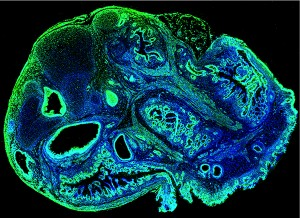
\includegraphics[width=0.8\columnwidth]{figures/cerebral_organoid/cerebral-organoid-for-Broad-web-300x218}
\caption{A cerebral organoid viewed under fluorescence microscopy \citep{nguyen_wang_nikolakopoulou_2015}.%
}
\end{center}
\end{figure}

\subsection{Brain development}

The mammalian brain is among the most complex organized structures in biology. The development of the animal nervous system, termed neural induction, is initiated by the formation of several primitive cell clusters early in development. This initial differentiation of neural progenitors begins with the formation of the neural plate on the ectoderm (outer layer) of the embryo, which folds inward to form the neural fold/groove, creating the neural tube and crest (Figure~\ref{fig:development}). 

\begin{figure}[h!]
\begin{center}
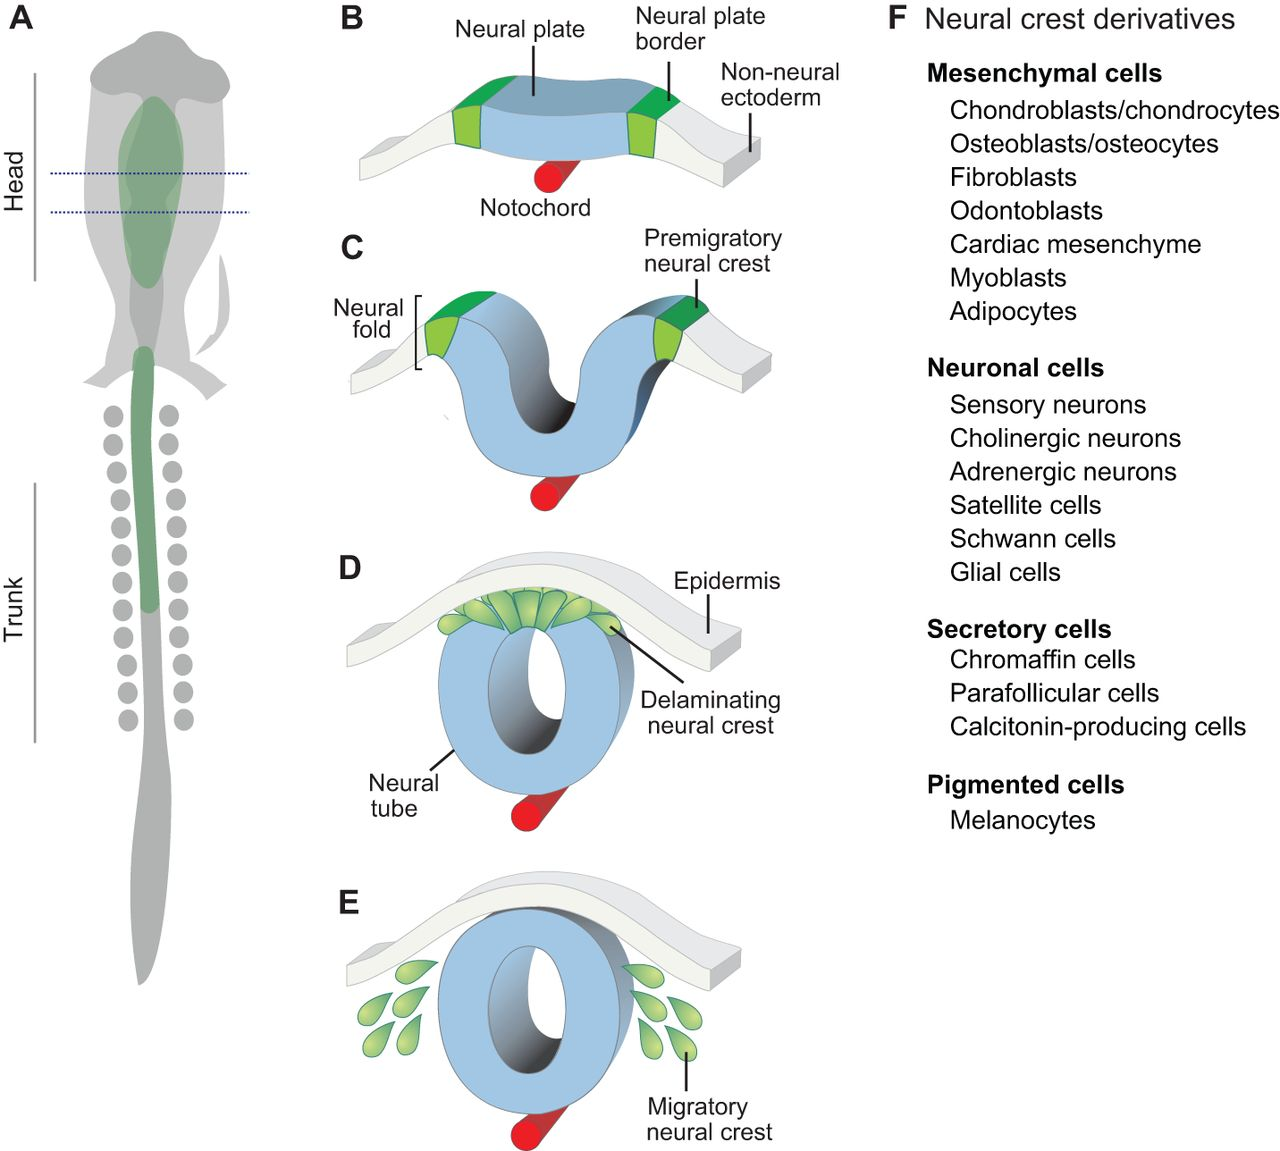
\includegraphics[width=0.8\columnwidth]{figures/brain_development}
\caption{Development of the neural tube \citep{neural_development}. \label{fig:development}%
}
\end{center}
\end{figure}

The neural tube is characterized by four regions which develop into distinct adult structures \citep{Bakken_2015}. The first of these, the prosencephalon, develops into the telencephalon and diencephalon, which further develop into the forebrain, hypothalamus, and eyes. The second region, the mesencephalon, develops into the midbrain. The third region, the rhombencephalon (named for its rhombus-like shape), is responsible for the lower regions of the brain such as the cerebellum, pons, and medulla oblongata, which originate from the metencephalon and myelencephalon. The last of these regions is the spinal chord.

\subsection{Gene expression regulation}\label{regulation}
Gene expression at the cellular level is regulated by a plethora of molecular means and is the foundation of an organism's development, growth, and survival. Although the vast majority of cells (except germ and certain immune cells) in an animal have identical DNA, their own structure and function is determined by these methods of regulation. This cellular regulation further determines the structure and function of the upper-level tissues, organs, and ultimately the organism itself. 

Gene expression consists of the processes of DNA transcription to RNA and RNA translation to the amino acid chain that becomes the protein. Transcription is influenced by transcription factors, which affect how well an RNA polymerase (the enzyme primarily responsible for transcription) is able to bind to and form a transcription complex on a gene. Specific examples of molecules affecting gene expression include the addition of acetyl or methyl groups to the DNA and proteins that by binding to the DNA, can either attract or block the binding of RNA polymerase. In eukaryotic cells such as those of mice and humans, the RNA transcript must be further processed prior to transcription. This post-transcriptional processing involves the addition of cap and tail sequences that protect the sequence from digestive enzymes and allow for translation to occur. The RNA transcript also contains exon and intron regions; only the exon regions are incorporated into the final sequence to be translated. Once the RNA transcript has left the nucleus of the cell (through a nuclear pore), a ribosome (a large cellular machine that facilitates translation of RNA to protein) binds to the RNA and initiates construction of the amino acid chain. Once the amino acid chain is complete, the ribosome splits in two, and the protein may be further modified. For instance, the chain may be folded within a chaperonin, which oversees the formation of the correct conformational design for some proteins, or the protein may be tagged with small molecules that identify its destination. These methods, and many others, allow for extremely precise regulation of complex genetic pathways that are the drivers of embryonic development.

The embryonic phase of development is known for highly dynamic expression of genes across time and space, or spatiotemporal regulation. Differential gene expression over space and time is the feature that allows an organism to develop specialized cells. Conditional regulation of only a  select few high-level "master genes" can determine the fate of a cell. 
\citep{bisceglia_2010}

\begin{figure}[h!]
\begin{center}
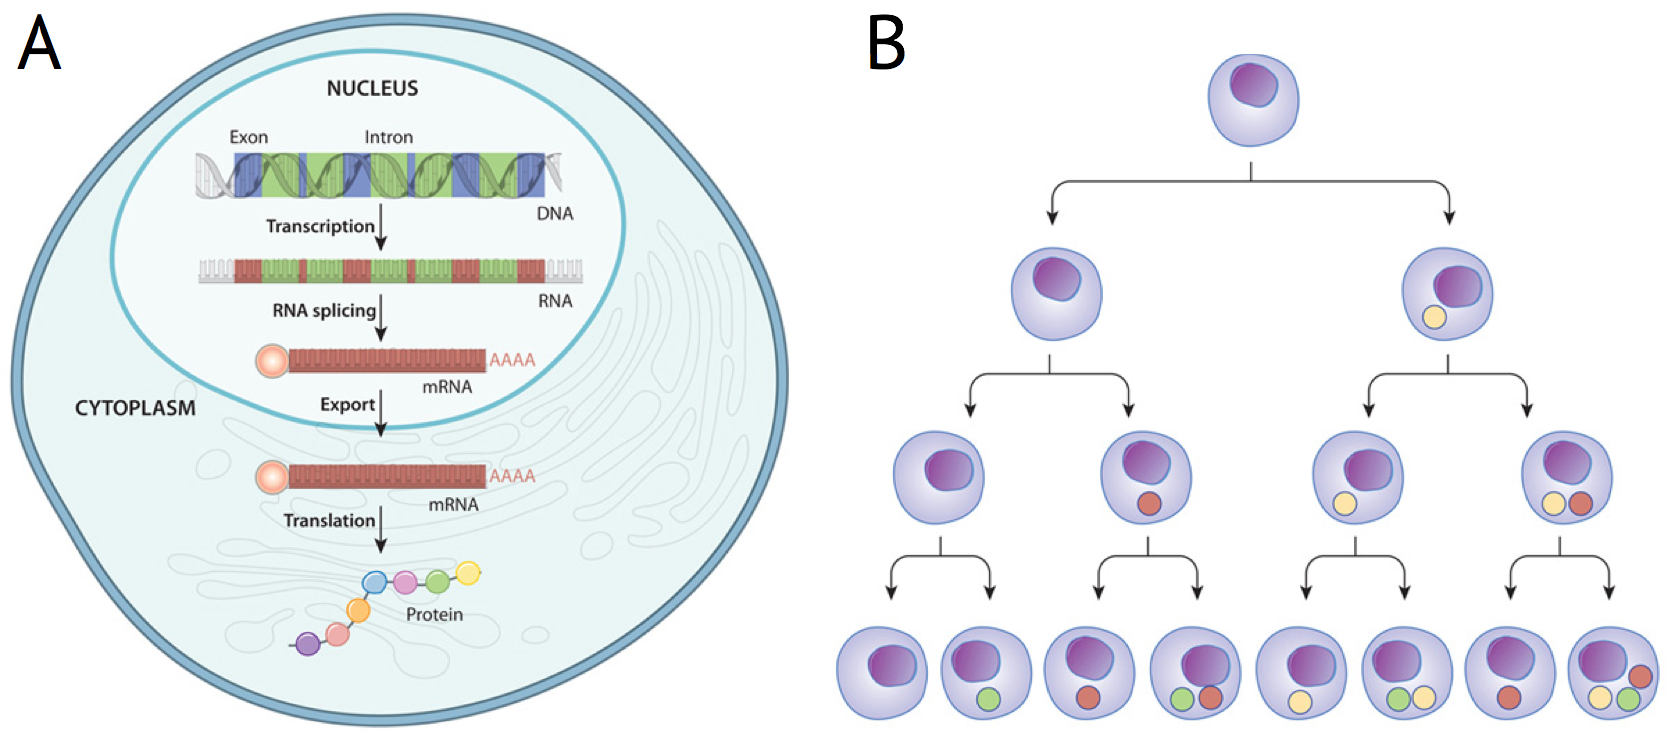
\includegraphics[width=0.8\columnwidth]{figures/Untitled/Untitled}
\caption{\textbf{A.} A general overview of the flow of information from DNA to RNA to protein. \textbf{B.} Demonstration of cell differentiation \citep{bisceglia_2010}.%
}
\end{center}
\end{figure}

\subsection{Gene expression measurement}
Numerous methods exist for the quantification and visualization of gene expression data. Two established methods include \textit{in situ} hybridization (ISH) or RNA sequencing (RNA-Seq). 

ISH is a technique that allows specific sequences of nucleic acids to be located in a section of cells or tissue. This localization is accomplished through the principle that complementary nucleic acid sequences form hydrogen bonds (hybridize) with each other. The complementary sequence, or the \textit{probe}, that detects the target sequence may be identified through fluorescent (fluorescent DNA components), radioactive (radioactive isotopes), or immunohistochemical (antibody-labeled) means. After the probe is allowed to hybridize to the target strand, RNases (RNA-digesting enzymes) hydrolyze any excess probes and the rest are washed off, leaving only bound probes behind. Following ISH, fluorescent microscopy may then be used to highlight regions of gene expression, which may then be scanned and analyzed using image analysis algorithms \citep{Angerer_1991}. Regions of high expression of the sequence of interest are shown as darker areas in an image (Figure~\ref{fig:ish}). 

In addition to ISH, RNA-Seq is also used in order to accurately measure gene expression. Because the primary function of RNA in the cell is as an intermediate in the transfer of information from DNA to protein, RNA expression levels can give an approximate indication of overall gene expression levels. In RNA-Seq, as the name suggests, next-generation nucleic acid sequencing is applied to a collection of RNA sampled from a tissue region. This RNA sample is first isolated from the source tissue through digestion using detergents and enzymes. Once the RNAs are isolated, a next-generation sequencing machine reads all the RNA to a digital storage device. These raw sequence data are then formatted to identify exons and introns, which may be later used to identify gene expression levels. These gene expression values provide an approximate indication of the degree of a gene's expression within a cell \citep{Wang_2009}.

\begin{figure}[h!]
\begin{center}
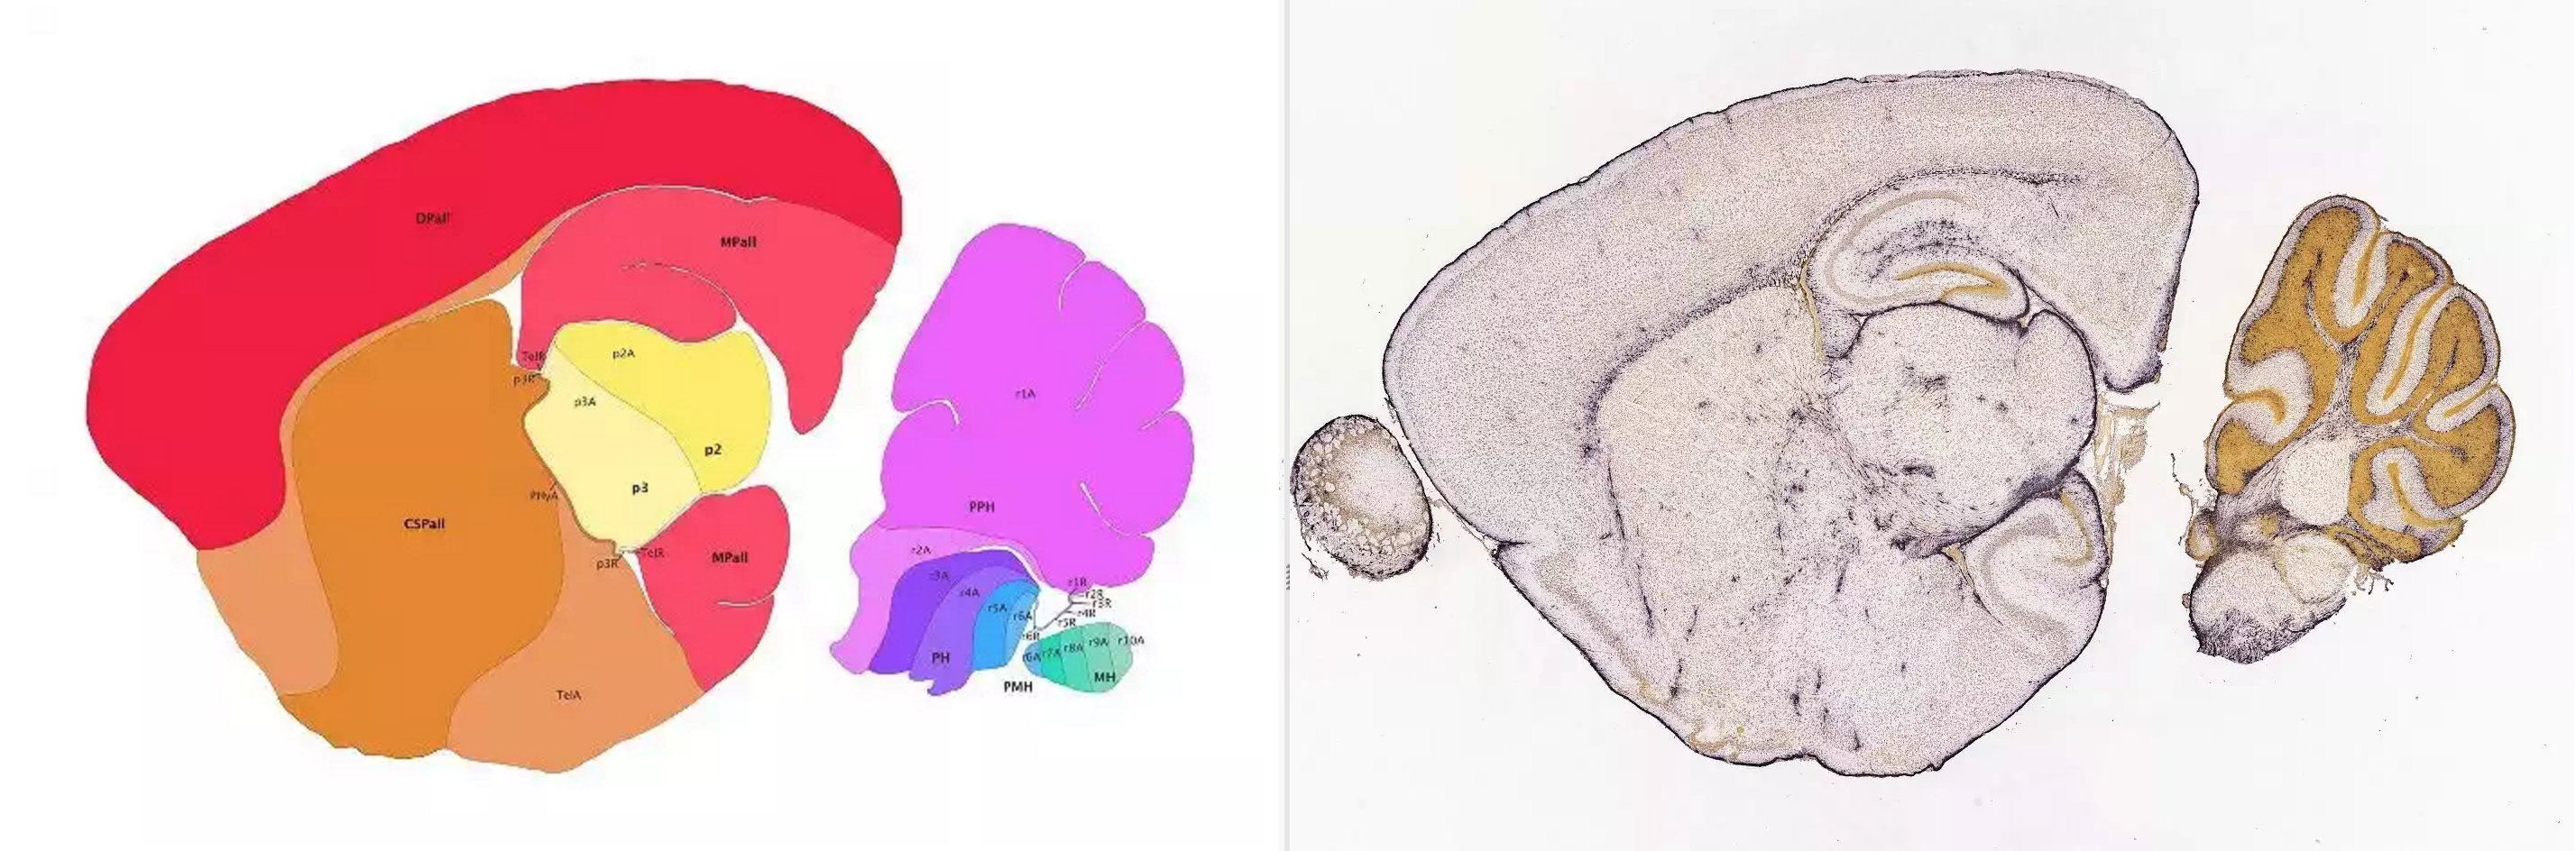
\includegraphics[width=0.8\columnwidth]{figures/ISH/ISH}
\caption{An ISH stain for glial fibrillary acidic protein (GFAP) RNA in the P14 mouse brain. At left is a diagram of the regions shown in the staining for reference (Allen Brain Atlas).\label{fig:ish}
}
\end{center}
\end{figure}

\subsection{Gene expression analysis}\label{gene_analysis}

Gene expression values offer valuable insights into the dynamics of regulatory networks and cellular processes. Analyses may be performed at any level of regulation described in Section~\ref{regulation}. Among one of the most widely used expression analysis techniques are those which cluster genes by similarity of expression. These methods can be used to generate dendrograms (Figure~\ref{fig:leukemia}) that provide a hierarchical ordering of the genes. Genes within a cluster are assumed to share a common underlying biological mechanism of action that is responsible for similar expression patterns.

The accuracy of a clustering depends heavily on the hyperparameter $K$, which denotes the number of clusters. In hierarchical clustering, a certain value of $K$ is equivalent to cutting the produced dendrogram at a certain level. An excessively low $K$ may lead to large clusters which provide an overly general fit to the genes and fails to provide any meaningful insight. An excessively high $K$, on the other hand, may create more clusters than is necessary and creates categories where there are none. The validity of the clustering may be assessed by removing one of the predictor variables (for instance, a specific timepoint or region of expression), and examining whether or not the resultant clustering is significantly altered \citep{how_expression_works}. A significantly altered clustering would suggest that one variable affects the clustering to an abnormal degree, which may imply that the clustering method is chaotic.

\begin{figure}[h!]
\begin{center}
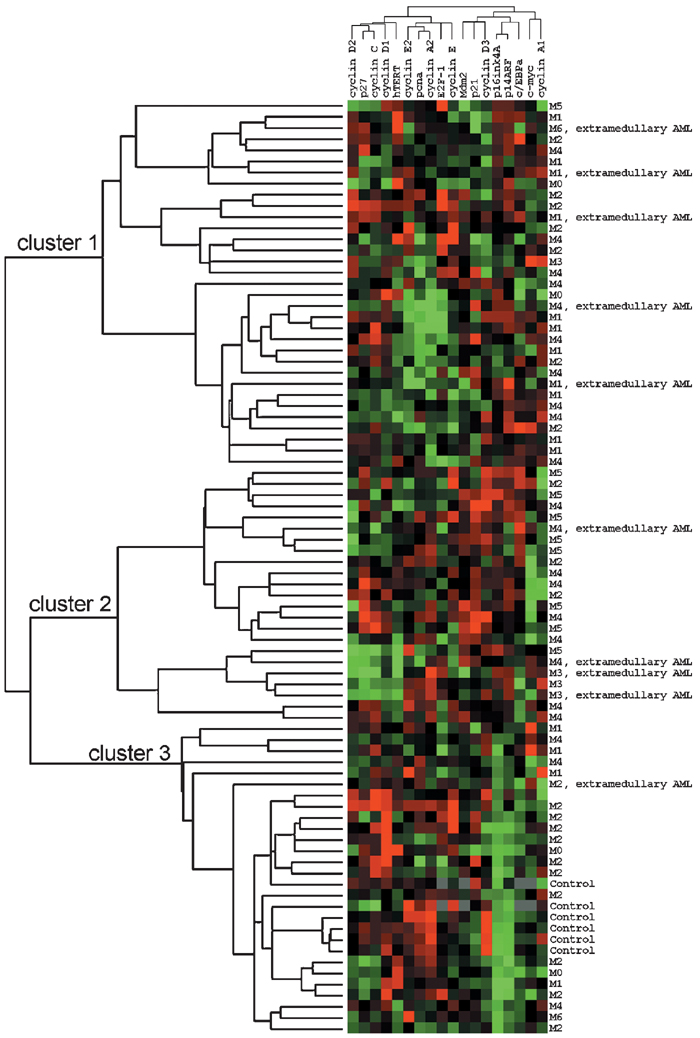
\includegraphics[scale=0.25]{figures/leukemia_clustering}
\caption{An example of a clustering algorithm applied to expression values of genes related to acute myeloid leukemia. Dendrograms were created for regions (top) and sample (left) \citep{leukemia_clustering}.\label{fig:leukemia}
}
\end{center}
\end{figure}

\subsection{The Allen Brain Atlas}
Founded in 2003 by Microsoft co-founder Paul Allen, the Allen Institute for Brain Science is a nonprofit research organization dedicated to the public pursuit of brain research. Among the many free datasets provided by the Institute are the Allen Developing Mouse Brain Atlas (located at \href{http://www.developingmouse.brain-map.org/}{www.developingmouse.brain-map.org/}) and the Allen Atlas of the Developing Human Brain (located at \href{http://www.brainspan.org/}{www.brainspan.org/}).

The Developing Mouse Brain Atlas features in situ hybridization (ISH) data for over 2,100 genes across multiple stages of embryonic and postnatal mouse brain development. The raw images of the ISH scans total 434,946 images. These images were assembled into 3-dimensional grids of expression values.  In addition, an application programming interface (API) in the form of a bioinformatics pipeline allows researchers to access all data produced by the Developing Mouse Brain studies. The Developing Mouse API further allows researchers to obtain quantized expression values per region, which are calculated based off of analysis of the ISH scan images. These expression values may be found for several different developmental time points, at several discrete brain regions, for each of the 2,100+ genes \citep{Thompson_2014}.

Similar to the Developing Mouse Brain Atlas, the Developing Human Brain Atlas also features a diverse array of ISH expression values for several thousand genes. These expression values are available for download as raw comma-separated-values (CSV) files from the Developing Human Brain Atlas Website, although an API is still available. In addition to ISH images, extremely detailed, cellular-level, magnetic resonance imaging (MRI) and microarray data are also included \citep{24695229}. The expression levels for these images may be summarized using image analysis techniques provided by the Brain Atlas API which yield region-time expression matrices (Figure~\ref{fig:matrix}).

\begin{figure}[h!]
\begin{center}
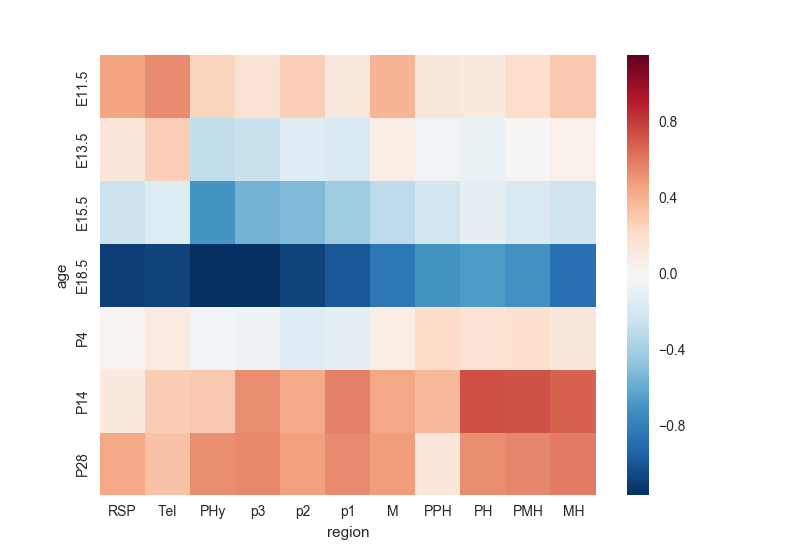
\includegraphics[width=0.8\columnwidth]{figures/Abl1/Abl1}
\caption{A heatmap of expression values for the Abelson murine leukemia viral oncogene homolog 1 (ABL1) gene in the developing mouse brain. Expression values were obtained from ISH stains and computed for each region using specialized 3-D voxel counts provided by the Allen Brain Atlas API. The y-axis is the development stage and the x-axis is the brain region (abbreviated). The expression values were transformed to a logarithmic scale to account for skew. \label{fig:matrix}%
}
\end{center}
\end{figure}

\subsection{Neural networks}
Neural networks are a subfield of machine learning, which is often cited as the ``field of study that gives computers the ability to learn without being
explicitly programmed," a definition given by Arthur Samuel in 1959. Although invented around the mid 19-th century \citep{Zilouchian2001FundamentalsON}, neural networks today are one of the most flexible and powerful machine learning algorithms. In several areas of research, neural networks offer state-of-the-art performance over traditional, hand-coded methods, such as in image pattern recognition, genomic analysis, and protein folding prediction. The basic neural network node, or \textit{neuron}, is similar to its biological counterpart in that it receives a number of inputs and outputs an output (Figure~\ref{fig:neuron}). However, the two differ in both structure and function. For instance, the biological neuron asynchronously receives a combination of excitatory and inhibitory impulses and sends a constant output signal. An artificial neuron instead is a mathematical construct that receives inputs synchronously and usually has a variable output value. In addition, whereas biological neural networks tend to be complicated in their topologies (many are not yet understood), artificial neural networks almost always have a tree-based structure of connectivity. The two further differ in their application: whereas brains are capable of extrapolation and learning of novel tasks, artificial neural networks are specialized and cannot readily adapt to new tasks given learned information.

\begin{figure}[H]
\begin{center}
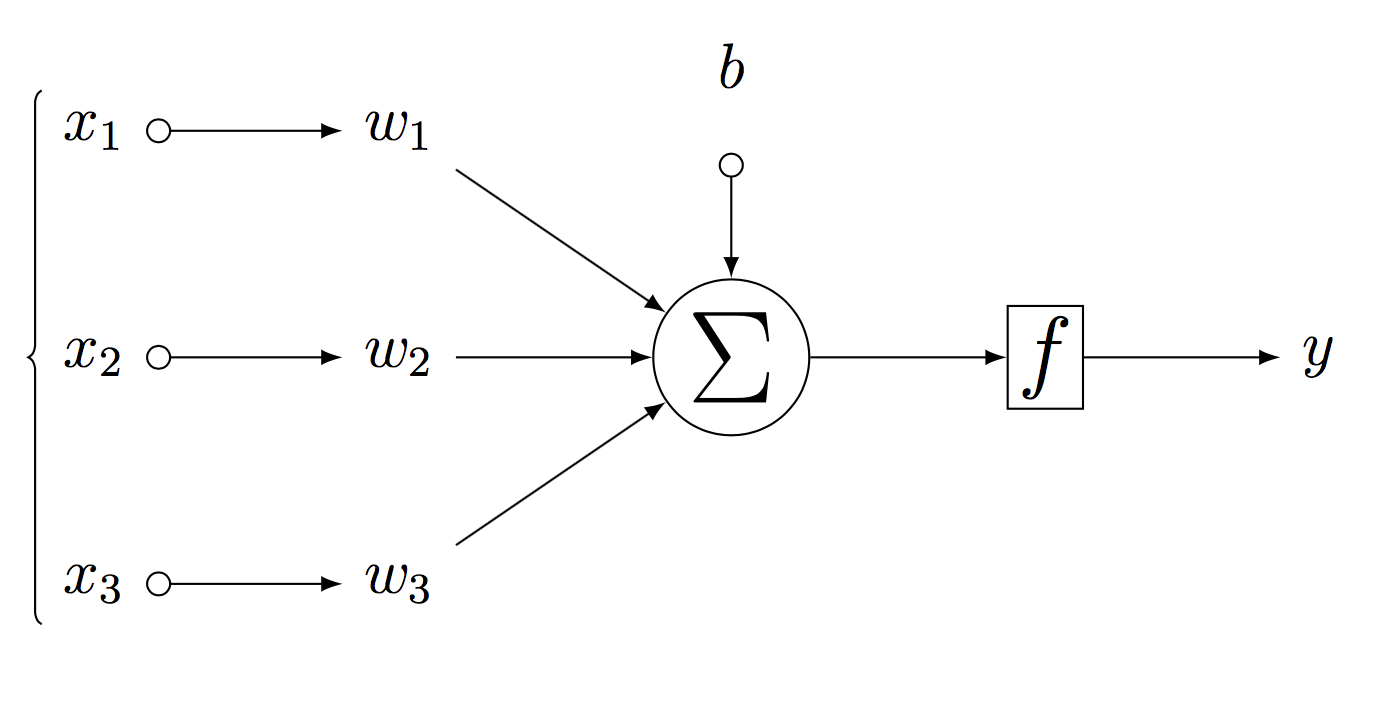
\includegraphics[width=0.8\columnwidth]{figures/neuron}
\caption{A diagram of a basic neuron with input values $x_{1}$,$x_{2}$, and $x_{3}$ with respective weights $w_{1}$,$w_{2}$, and $w_{3}$ and a bias $b$. The neuron computes the sum of these inputs and outputs a value $y$ determined by activation function $f$. \label{fig:neuron}}
\end{center}
\end{figure}

Neural networks learn by minimizing an objective function which determines the degree of error present in the predictions of a network. This gradual minimization is done by adjusting the specific weights and biases in a network. When a network is first initialized, the weights present are usually set to zero or randomly determined using a probability distribution function. As the network is fed data, the outputs are compared to target values and a loss value is computed. This loss value is then used to adjust the weights of the network to better fit the inputs to the output using a method called backpropagation in which the effect of each neuron on the loss function is computed using the chain rule. The weights are then updated using a method of gradient descent in order to minimize the loss value. This iterative updating allows the network to eventually learn a complex function given enough training data and time \citep{Zilouchian2001FundamentalsON}. 

There exist a multitude of activation functions which determine the output of an artificial neuron (Figure~\ref{fig:activations}). Many of these functions are designed such that the loss gradients have smooth derivatives that can be handled by backpropagation. For instance, a step function would not be able to be backpropagated. The activation functions will also partly determine the computational workload; a ReLU activation gradient, having a constant derivative, requires less processing power than a sigmoid activation gradient.

\begin{figure}[H]
\begin{center}
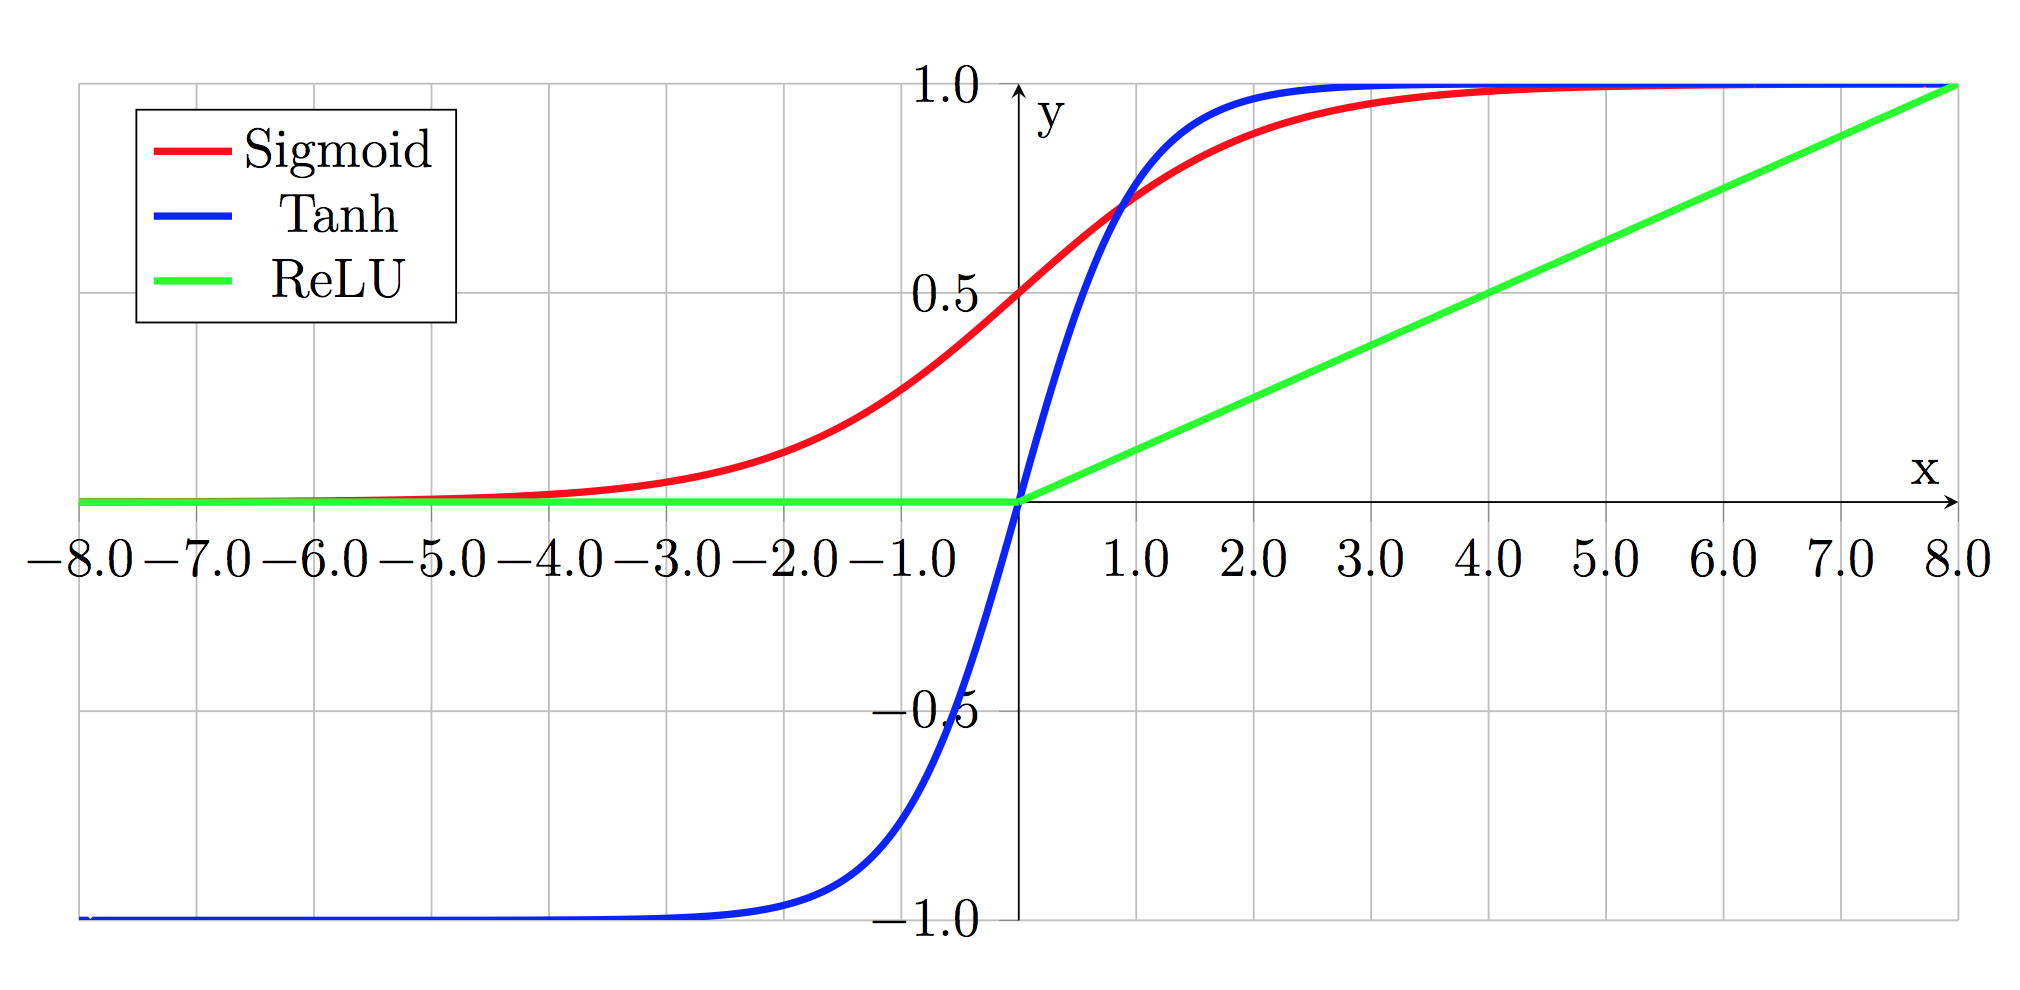
\includegraphics[width=0.8\columnwidth]{figures/activations}
\caption{Graphs of common neuron activation functions.\label{fig:activations}}
\end{center}
\end{figure}

\begin{table}[H]
\begin{center}
\caption{Equations of the activation functions shown in Figure~\ref{fig:activations}.}
\begin{tabular}{ l | l | l | l }
 Linear & Sigmoid & Tanh & ReLU\\ 
 $a(x) = x$ & $a(x) = \frac{1}{1+e^{-x}}$ & $a(x) = \frac{e^{x}-e^{-x}}{e^{x}+e^{-x}}$ & $a(x) = 0\ \textrm{if}\ x \leq 0, x\ \textrm{if}\ x > 0$\\   
\end{tabular}
\label{table:1}
\end{center}
\end{table}

Neural networks are able to approximate complex functions such as classifiers through abstraction by multiple layers. In general, larger neural networks tend to yield more accurate predictions and lower losses. However, large networks are very computationally expensive to train and may also overfit the data when there are not enough training examples \citep{Zilouchian2001FundamentalsON}.

\begin{figure}[H]
\begin{center}
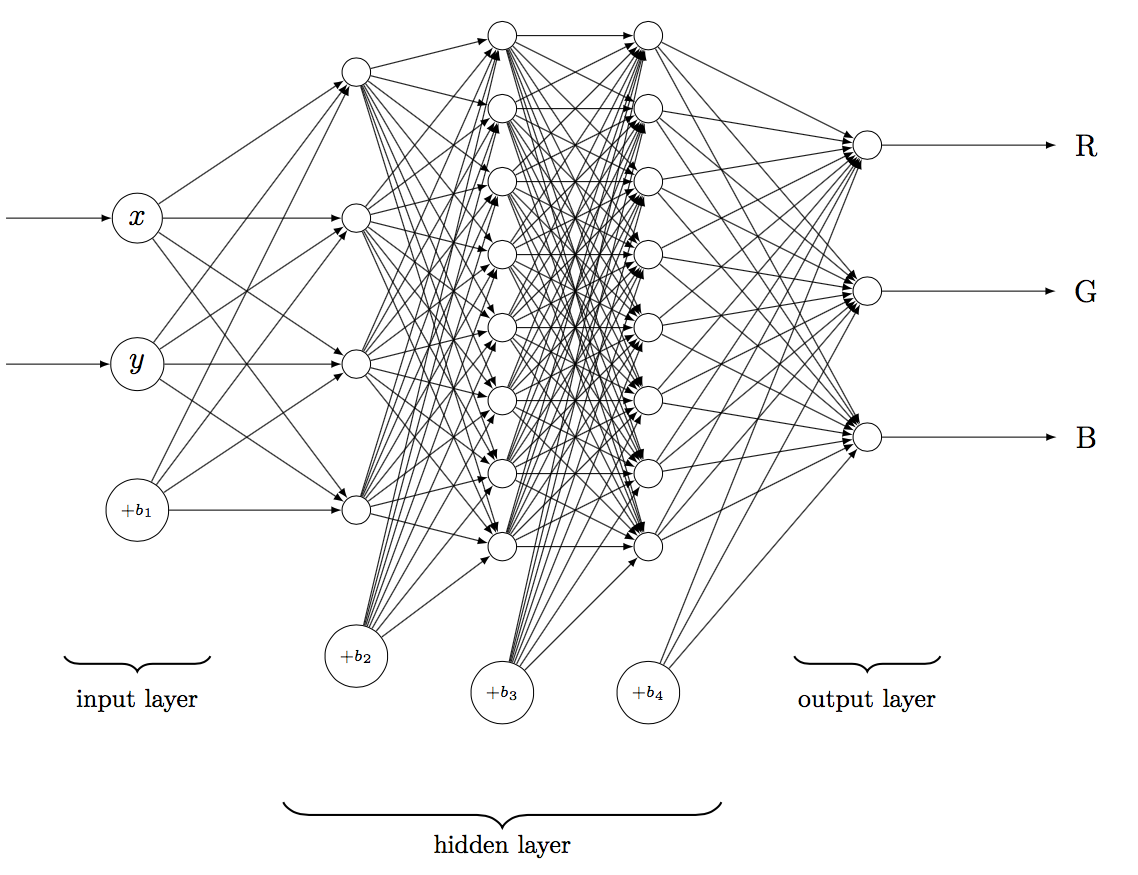
\includegraphics[width=0.8\columnwidth]{figures/doodle}
\caption{An example neural network that learns to generate an image given x and y pixel position inputs. The inputs are the x and y coordinates of the pixel, and the outputs are the three red-green-blue (RGB) values that define the color of a pixel.
\label{fig:doodle}
}
\end{center}
\end{figure}

In image analysis, a specific type of neural network termed the convolutional neural network is often used. Convolutional neural networks are loosely based on the structure of the animal visual cortex, which contains overlapping receptive fields. Similarly, in the convolutional neural network architecture, the inputs to a neuron are shared, convolving the input image. In a convolutional layer, the inputs are processed using filters, which are the two-dimensional representations of the weights used by each unit, or kernel, of the layer. These filters are gradually adjusted during training to recognize specific features in the input. The results of the convolution are then processed using a pooling method (Figure~\ref{fig:convolutional_mnist}) that produces a more abstract representation. In deep learning, convolutional and pooling layers are often coupled in a sequence such that higher level features may be learned from the data. For example, while the first layer of convolution may be trained to recognize edges, later layers may recognize shapes and eventually discrete objects. The primary advantage of convolutional neural networks lie in the fact that they are locally scale-invariant: convolution allows a feature of the image to be recognized regardless of position \citep{Krizhevsky2012ImageNetCW}.

\begin{figure}[H]
\begin{center}
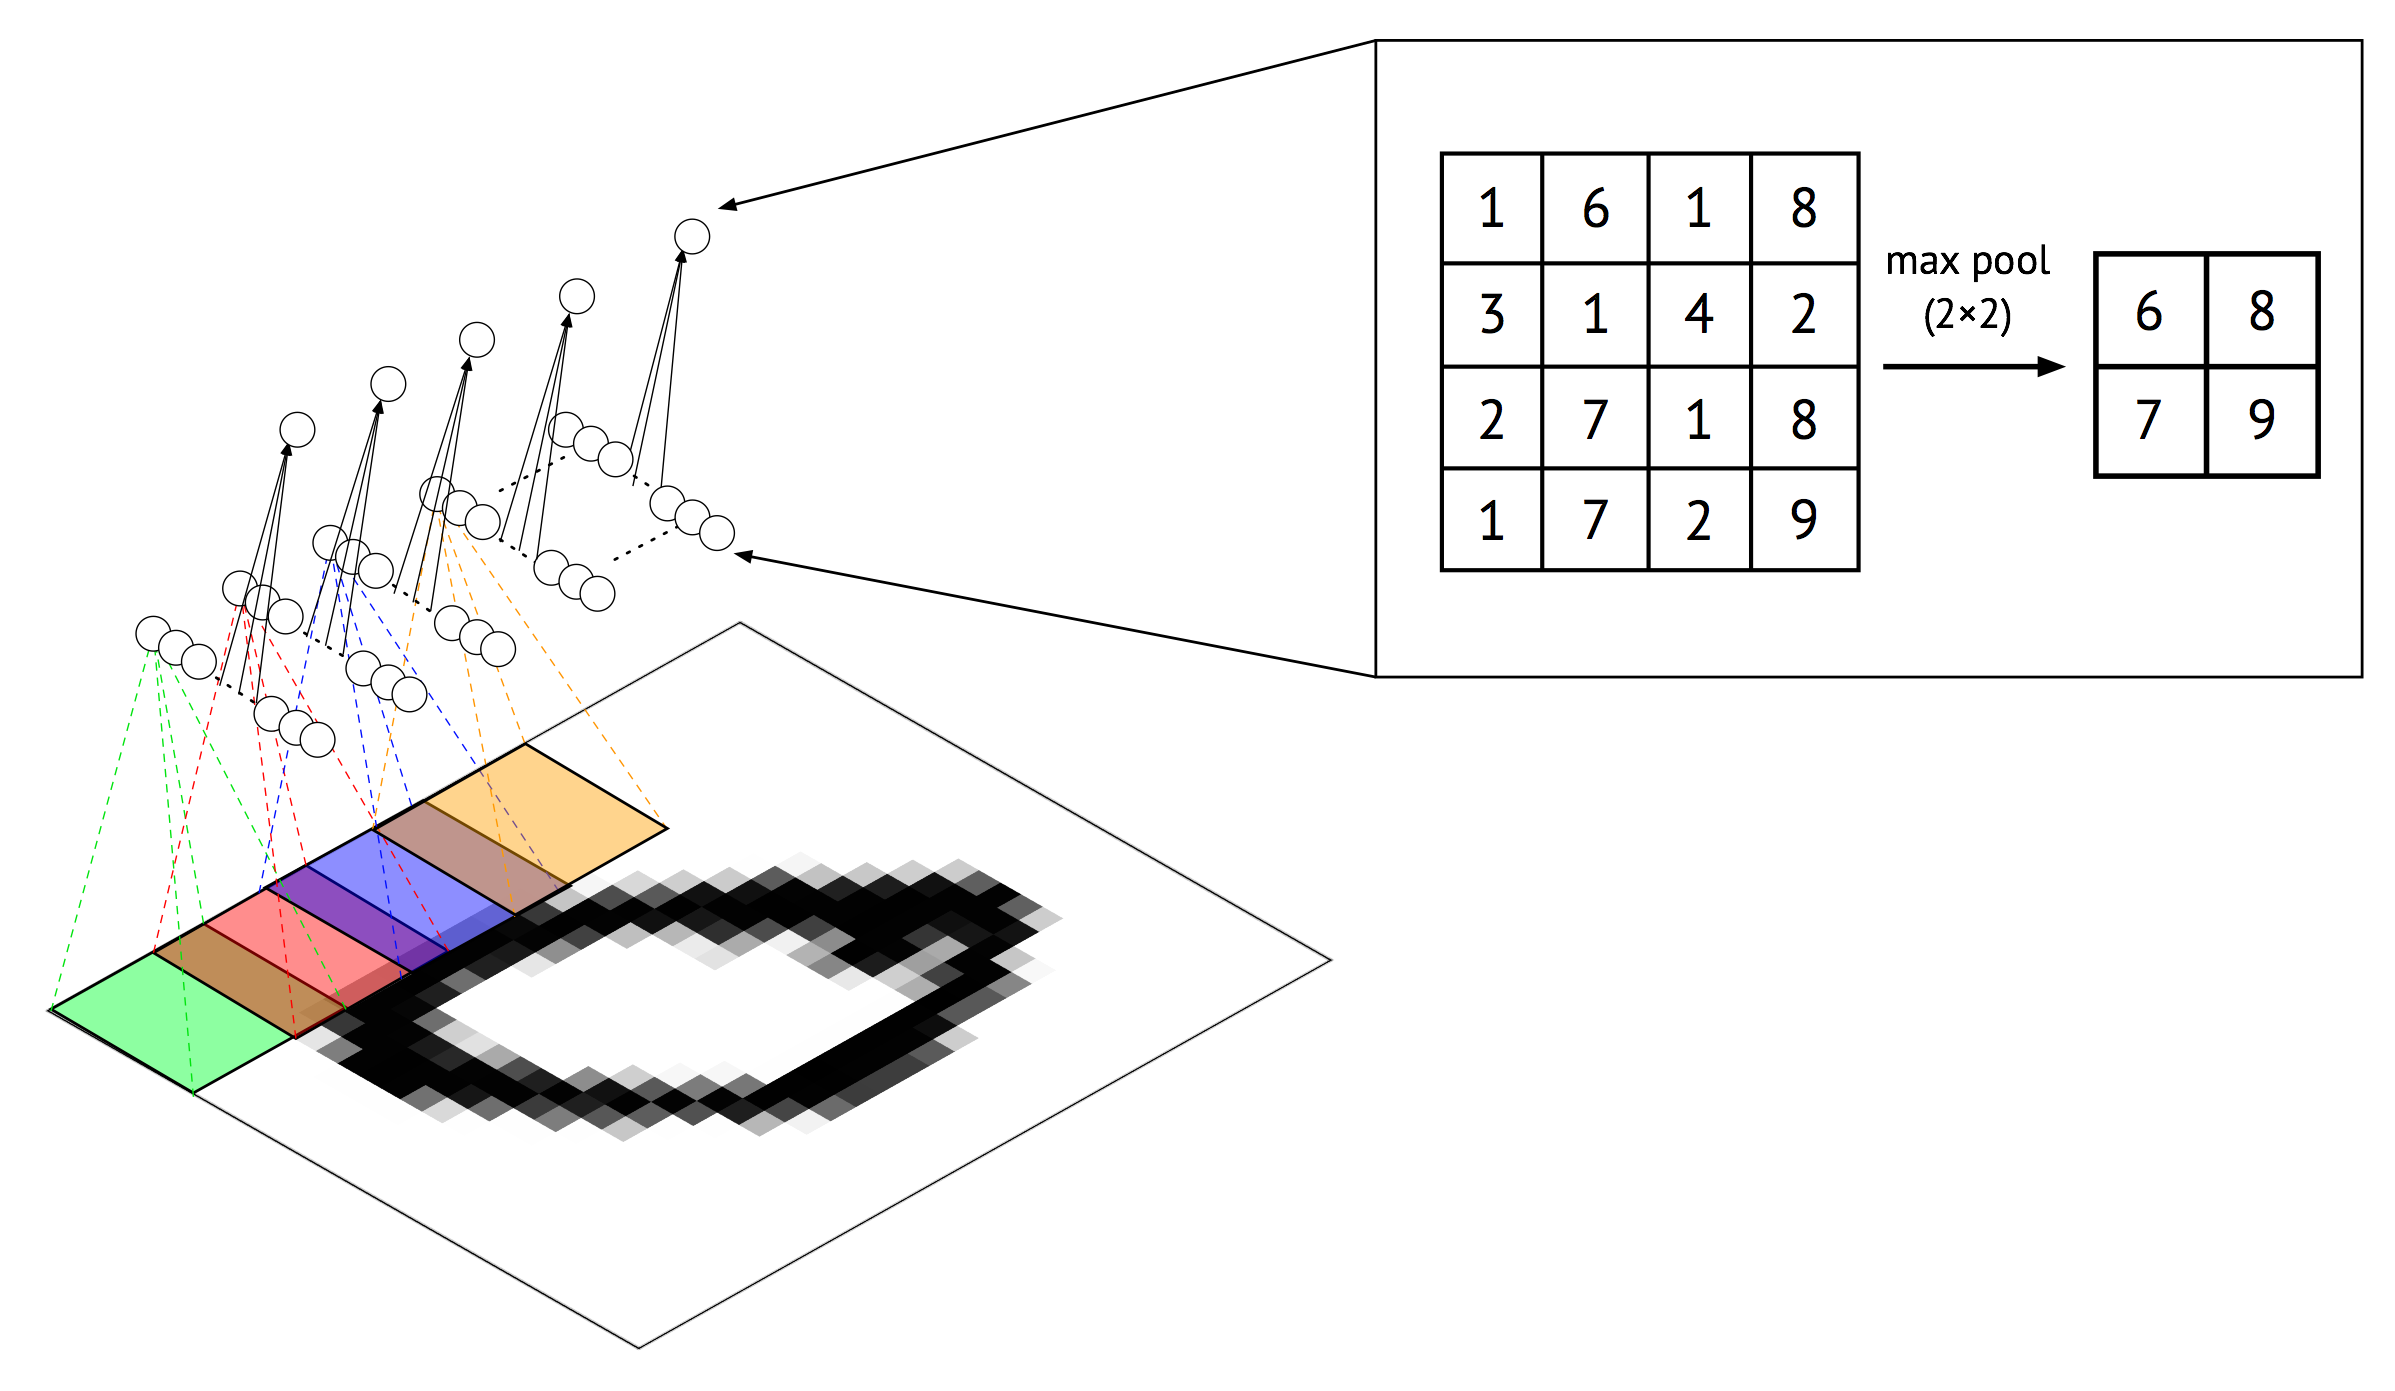
\includegraphics[width=0.8\columnwidth]{figures/convnet}
\caption{An example of a simple convolutional network designed for digit classification of the MNIST dataset. \label{fig:convolutional_mnist}}%
\end{center}
\end{figure}

Following convolution and pooling layers, a traditional dense layer of neurons is implemented to classify the features obtained (Figure~\ref{fig:mnist_full}). Variations of these networks are currently considered state-of-the-art in nearly all image classification tasks \citep{Koushik2016UnderstandingCN}.

\begin{figure}[H]
\begin{center}
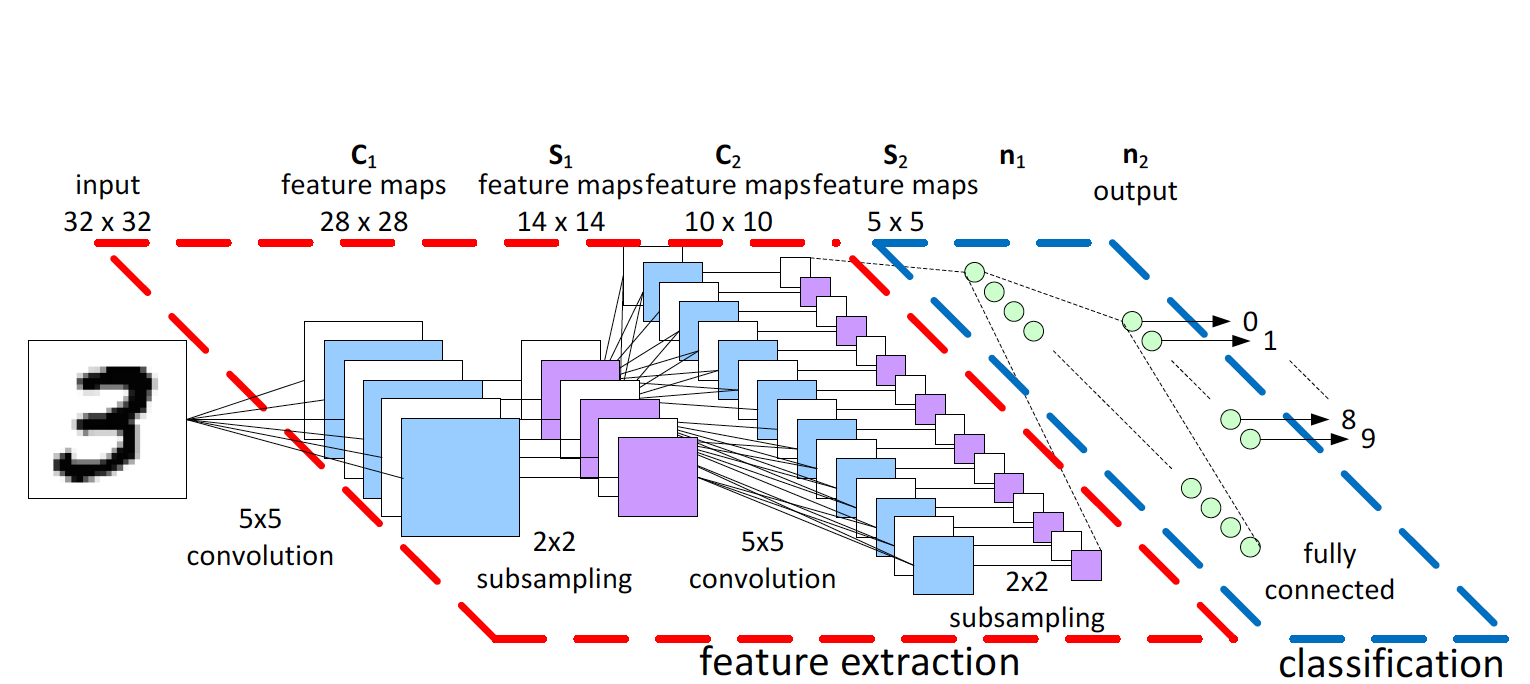
\includegraphics[width=0.8\columnwidth]{figures/CNN/CNN}
\caption{An example of a multi-layer CNN for classifying handwritten digits from the MNIST dataset. The feature extraction section repeatedly convolves the input image to higher level features, which are fed as inputs to the classification stage. In this case, the classification stage is composed of two fully connected layers, with the final layer outputting the predicted digit classification \citep{peemen_mesman_corporaal_2011}. \label{fig:mnist_full}%
}
\end{center}
\end{figure}

\subsection{Unsupervised learning}

Machine learning can be divided into the two subfields of unsupervised and supervised learning. The primary difference between the two is in the training of the model: supervised learning trains the model using a predefined set of classifications, or \textit{labels}, unsupervised learning trains the model without such guidance. Figure~\ref{fig:super} gives a basic illustration of the difference between the two:
in the left diagram, the datapoints are labeled as being red hexagons or blue triangles. With these labels, one could train supervised programs such as classifiers that predict the label of a data point given its x-y position. On the figure on the right, however, none of the datapoints are labeled (all of them are red hexagons). For these data, one could apply an unsupervised method such as a clustering analysis program to group datapoints by how similar they are to each other. This allows researchers to make inferences regarding patterns and structures in the data.

\begin{figure}[H]
\begin{center}
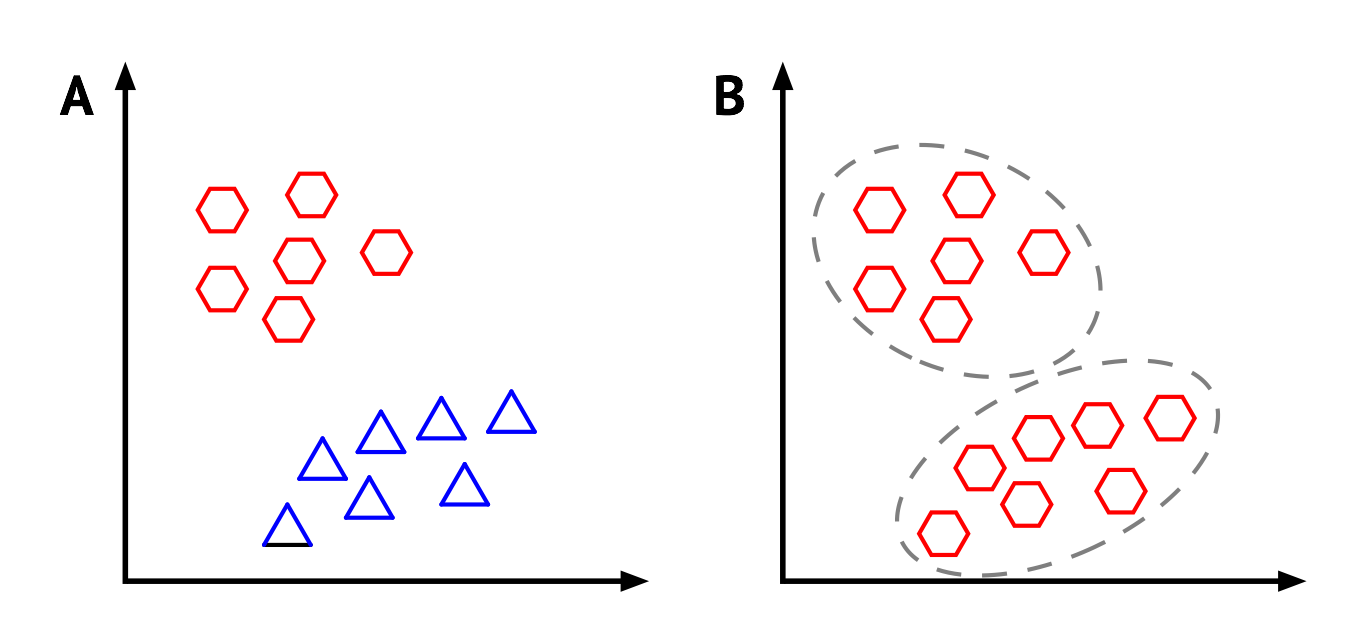
\includegraphics[width=0.8\columnwidth]{figures/learningtypes}
\caption{An illustration of the primary difference between supervised (\textbf{A}) and unsupervised (\textbf{B}) learning.\label{fig:super}
}
\end{center}
\end{figure}

Clustering is an essential method of unsupervised learning. Clustering analysis is often performed following dimensionality reduction methods that allow the data to be reduced to a simple two or three-dimensional representation while maintaining the original variance and structure in the data. Algorithms such as K-means, DBSCAN, and complete linkage clustering may then be employed to calculate clusters. In image classification tasks, classification and dimensionality reduction allow the learned results of a neural network to be visualized (Figure~\ref{fig:clusters}). Furthermore, a convolutional neural network may be directly coupled with a clustering algorithm as a loss function in order to gradually produce high quality clusters as the network is trained \citep{yangCVPR2016joint}.

\begin{figure}[H]
\begin{center}
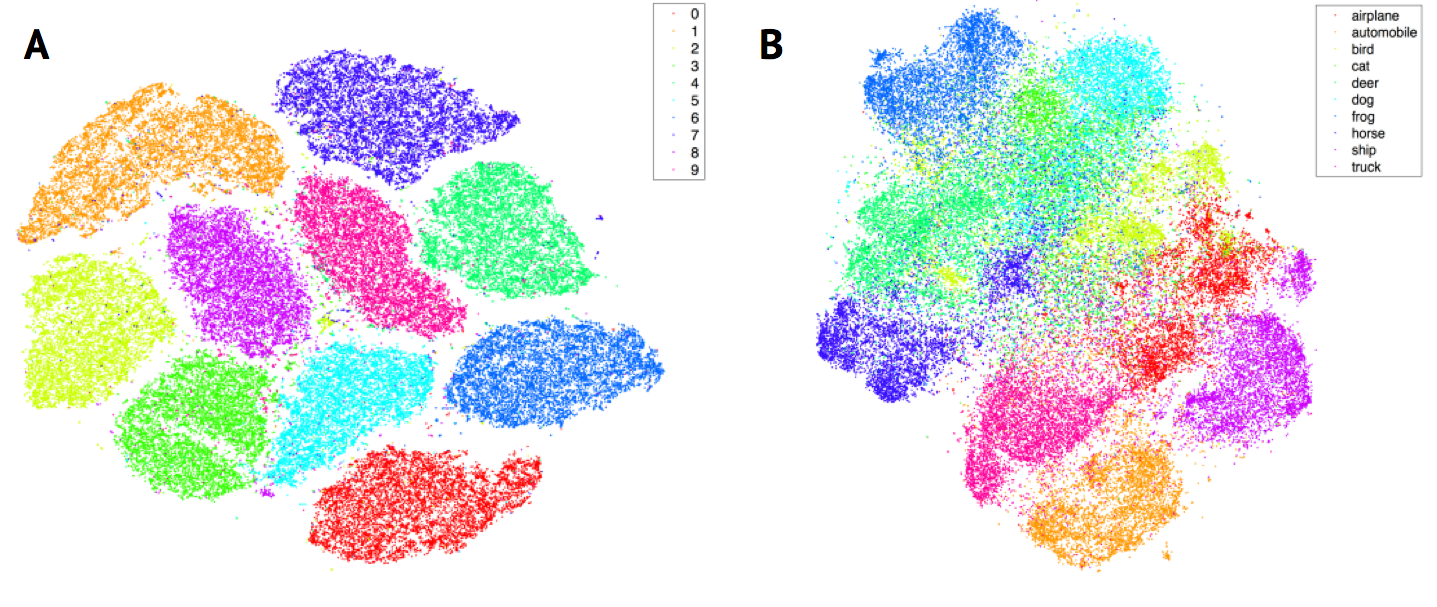
\includegraphics[width=0.8\columnwidth]{figures/tsne}
\caption{The results of a t-Distributed Stochastic Neighbor Embedding (t-SNE) dimensionality reduction on a clustering of the MNIST (\textbf{A}) and CIFAR-10 (\textbf{B}) datasets \citep{laurensvandermaaten2014}. \label{fig:clusters}%
}
\end{center}
\end{figure}

\section{Research plan}


\subsection{Researchable question}
Are there significant differences between patterns of gene expression in developing mouse and human central nervous systems?

\subsection{Hypothesis}

It is hypothesized that there exist significant differences between the gene expression profiles of developing mouse and human central nervous systems.

\subsection{Procedure}
This project will be entirely performed on a computer. Gene expression profiles for developing mouse and human brains will be first downloaded from the Allen Brain Atlas. Next, the data will be formatted and transformed into matrices of region versus time expression matrices. At this point, there will be two datasets, a developing human dataset and a developing mouse dataset. 

For each dataset, a convolutional neural network algorithm will be applied in order to automatically classify genes into discrete clusters based on patterns of expression. The relative positions of genes in the human and mouse clusterings will then be examined. Different clusterings would suggest that the transcriptomic landscapes is different. The gene expression clusterings may be applied to highlight discrete drug-gene interactions in human versus mouse brains. Potential differing expressions may account for anatomical differences in mouse and human brains. As a possible extension, the similarity of expression patterns in cerebral organoids will also be considered. The insights from this project may also be applied to single-cell cancer sequencing, where clustering analysis may be used to for the characterization and identification stages of cancer cell development.

\section{Methodology}

\section{Results}

\section{Discussion}

\section{Conclusions}

\section{Limitations}

\section{Extensions}

\section{Acknowledgments}

\bibliographystyle{apa}
\bibliography{bibliography/biblio.bib%
}

\end{document}

